\documentclass[IEEEtran,letterpaper,10pt,titlepage,fleqn,draftclsnofoot,onecolumn]{article}
%notitlepage vs titlepage
%fleqn left align

%\usepackage{nopageno} %no page numbers
\usepackage{indentfirst}
\usepackage{alltt}                                           
\usepackage{float}
\usepackage{color}
\usepackage{url}

\usepackage{graphicx}                                        
\usepackage{amssymb}                                         
\usepackage{amsmath}                                         
\usepackage{amsthm}                                          

\usepackage{balance}
%\usepackage[TABBOTCAP, tight]{subfigure}
\usepackage{enumitem}
\usepackage{pstricks, pst-node}
\usepackage{geometry}
\usepackage{hyperref}
\usepackage{textcomp}
\usepackage{listings}
%allows for code snipets

\geometry{textheight=9.5in, textwidth=7in} 

\newcommand{\cred}[1]{{\color{red}#1}} %think function call, changes text to red
\newcommand{\cblue}[1]{{\color{blue}#1}} %text to blue
\definecolor{dkgreen}{rgb}{0,0.6,0}
\definecolor{gray}{rgb}{0.5,0.5,0.5}
\definecolor{mauve}{rgb}{0.58,0,0.82}
\lstset{frame=tb,
  language=c,
  aboveskip=3mm,
  belowskip=3mm,
  showstringspaces=false,
  columns=flexible,
  basicstyle={\small\ttfamily},
  numbers=none,
  numberstyle=\tiny\color{gray},
  keywordstyle=\color{blue},
  commentstyle=\color{dkgreen},
  stringstyle=\color{mauve},
  breaklines=true,
  breakatwhitespace=true,
  tabsize=3
}
\setcounter{tocdepth}{4}
\setcounter{secnumdepth}{4}

\def\name{Brandon Ellis, Jiayu Han, and Jack Neff}
\def\class{CS 463}
\def\assignment{Spring Midterm Progress Report}

%PDF Properties
\hypersetup{
  colorlinks = true,
  urlcolor = black,
  pdfauthor = {\name},
  pdfkeywords = {CS463 Senior Capstone Spring Midterm Progress Report},
  pdftitle = {\class \assignment},
  pdfsubject = {\class \assignment},
  pdfpagemode = UseNone
}

\begin{document}
%TitlePage
\begin{titlepage}
  \begin{center}
    \vspace{1cm}
    
    \huge
    \textbf{Green Smart Gardening System: Spring Midterm Progress Report}
    
    \vspace{1.5cm}
    
    \large
        \textbf{Brandon Ellis, Jiayu Han, and Jack Neff}
    
    \vspace{5cm}
    
    Abstract
    
    \normalsize
    This document details the work done by the Green Smart Gardening Project (GS2) group. Our report is specifically on the work done during the first half of Spring Term. It is broken down by individual group members. Then, each group member will note the work they do, what they have left, any problems encountered so far this term, and then anything else of note will be mentioned.
    
    \vfill
    
    \large
        CS 463\\
        Spring Term\\
    \end{center}
\end{titlepage}

\section{Introduction}

The purpose of this report is to inform the reader about what the Green Smart Gardening System project has been working on. While the first half of Spring term is the main time frame, the report will have an all-encompassing feel. This is because each of the core pieces of are design document will be noted and covered. Brandon Ellis will note work done on air sensors, soil sensors, and board logic. Jack Neff will discuss work on the user interface, web application, and back-end database. Finally, Jiayu Han will cover the method of powering our device, WiFi, and the device’s packaging. To this end, each group member will be recapping work they are responsible for, where they are at with this work, what they will be working on for the duration of the term, and any interesting problems encountered along the way.

\section{Brandon Ellis}

\subsection{Introduction}

This report will detail what I have been doing for the beginning of Spring term. I will first be recapping the work that I have been assigned and what it entails. Then I will cover each of these pieces of work and discus where I am with them. The next section will detail work that I have left to do, specifically work prior to expo and the code freeze. Then, finally I will note some problems encountered and how they were valiantly defeated.

\subsection{Recap}

This section will discuss the work that I am responsible for in the GS2 team.

\subsubsection{Hardware Development}

The first responsibility that I have is hardware development. A main aspect of this comes in to play with the following section, regarding sensors. I am responsible for the wiring of our device. This mainly entails the sensors, but also requires me to work with the power side of things.

\subsubsection{Sensor Programming}

The second core responsibility I have is handling the sensors. There are three sensors used by our device. The first, by Adafruit, the BME280, this records air temperature, relative air humidity, and barometric pressure. The second sensor is dfrobot’s Capacitive Soil Moisture Sensor, which as its name suggest, records the moisture level in a given median. The final sensor is another by Adafruit, the GA1A12S202, which is notes the level of light. As hinted at in hardware development, a key part of my work is handling the physical hardware. For each of these sensors, I am in charge of soldering, wiring, and the embedded development required to communicate with each sensor.

\subsubsection{Board Logic}

The final job I have, is the rest of the embedded development. Once the communication to each sensor is in place, I am in charge of the other pieces of logic in play. This means setting up a time based schedule to do the following things. First connect to a network to facilitate transmitting recorded data. Gather said data from each sensor and then prepare it to be sent. Establish a communication with our server, and when that is in place, post the data to it. Request a page from the server that will contain a number. This number is a user specified time interval that the next run will be conducted on. Then, close the connection to our server. Finally, disconnect from the local network and hibernate until the next scheduled run.

\subsubsection{Testing}

While this is not one of my defined jobs, I have taken up testing the sensors and the functionality of our device. This means ensuring that data points recorded by each sensor are valid, and then making sure that our device can operate successfully over a long period of time.

\subsection{Where I Am}

\subsubsection{Hardware Development}

All hardware development has been completed. Most sensor wiring was done last time, but with the new sensor (which I will mention below) being received, I finished up the work by soldering pins to it and wiring it into our system.

\subsubsection{Sensor Programming}

All sensors have been successfully implemented. The last sensor we were waiting for was delivered just last week. With it I was able to, first test, then incorporate the GA1A12S202 Light Sensor into our full device. Once the data being recorded was fed into our server’s database, the final sensor requirement was met.

\subsubsection{Board Logic}

Everything mentioned in the board logic portion of the above Recap section has been finished. The scheduler is implemented based on first a hard-set time, then running off what the user has specified. During each scheduled run the board connects to a wireless network, connects to the server where it posts the collected data, checks what time interval it should run at, and then close down all active connections to go into sleep mode. Then it will wait a designated amount of time before starting that all over again.

\subsubsection{Testing}

To test our system, I have been running two types of tests. The first method is to test validity. To do this I have been testing our system against the environmental system in place at the OSU Green House. This way I can compare our data points against theirs to ensure that our sensors are accurate. The second test type done has been long running tests. These have been to make sure that our device, that is supposed to be running for a large period of time, can actually run for a large period of time. To do this I have been setting a low scheduled run time and multiple reading be noted and posted over a short period.

\subsection{What I Have Left}

\subsubsection{Long Running Test}

There are still some long running tests to be done. The main test is to hook up our system in its full power configuration with both the solar panel and its rechargeable batteries. This way, when I run it for a long period of time we can get an estimate at how fast the power is drained under different light levels.

\subsubsection{Test Suite}

While I have ensured the functionality of our board’s logic and the validity of the data transmitted, there is still work to be done to automate testing. Specifically, a program has already been developed to post static values to the database. These values will coincide with a script Jack wrote to check that said values were posted. This can provide us with some form of automation in our testing.

\subsubsection{Scheduler}

The final development related task I have to accomplish is the addition of a second scheduled task. This will be the last piece in solving the Two-Way Communication problem, described below. 

\subsection{Problems This Term}

\subsubsection{Changes to Power}

During this term we realized we had made a mistake recognizing which pins and ports on our MKR1000 where which. This specifically affected our arrangement of the solar panel in our wiring. Power from the solar panel would now feed through an unused, and intended for this purpose, Vin pin. Where the problem arose was in the ground line. No one in our team is really that familiar with the Electrical Engineering side of things. So, when the question of whether we could plug the ground from our solar panel, one of two forms of power at play, into the same breadboard circuit with the ground for our sensors, we didn’t have a definitive answer. I checked online to see if I could find a definite answer, but when I was unsatisfied with what I found (as it lacked concrete information), I was directed to the OSU TekBot Lab. I stopped by there and the technician was able to look over the problem at hand. She explained that plugging it in would be fine and that was the intended solution. She also explained why the ground was supposed to be along same circuit as the others. With newfound answers, we were able to move forward with powering the device.

\subsubsection{Two-Way Communication}

During this term we took on the task of setting up two-way communication between the device and the server. Originally, the board could only post information, but this was done through a http request that contained information. It was a simple fix to have a page containing information for the board to be set up, that the board could request. Then any information could be stripped from the downloaded webpage.

This technique was used to allow the user to specify a time. This number could then be retrieved by our board and used to update at what interval the scheduler runs at. The real problem here, and what is still to be done this term, comes from this functionality. It was pointed out that if the user set this for a very long time period, say multiple weeks, they would be unable to contact it or update the interval wirelessly until it came back online. My solution, which will be implemented this week, is a second scheduled task. The current, and only, task posts data and checks the time interval for itself. This new task would only check the interval for the first task, and possibly itself. This will create a sort of “check in” system that can not use as much power as the full task but can still check for updates.

\subsection{The Device}

\begin{figure}[H]
  \caption{GS2: Frolicking in the OSU Green House}
  \centering
  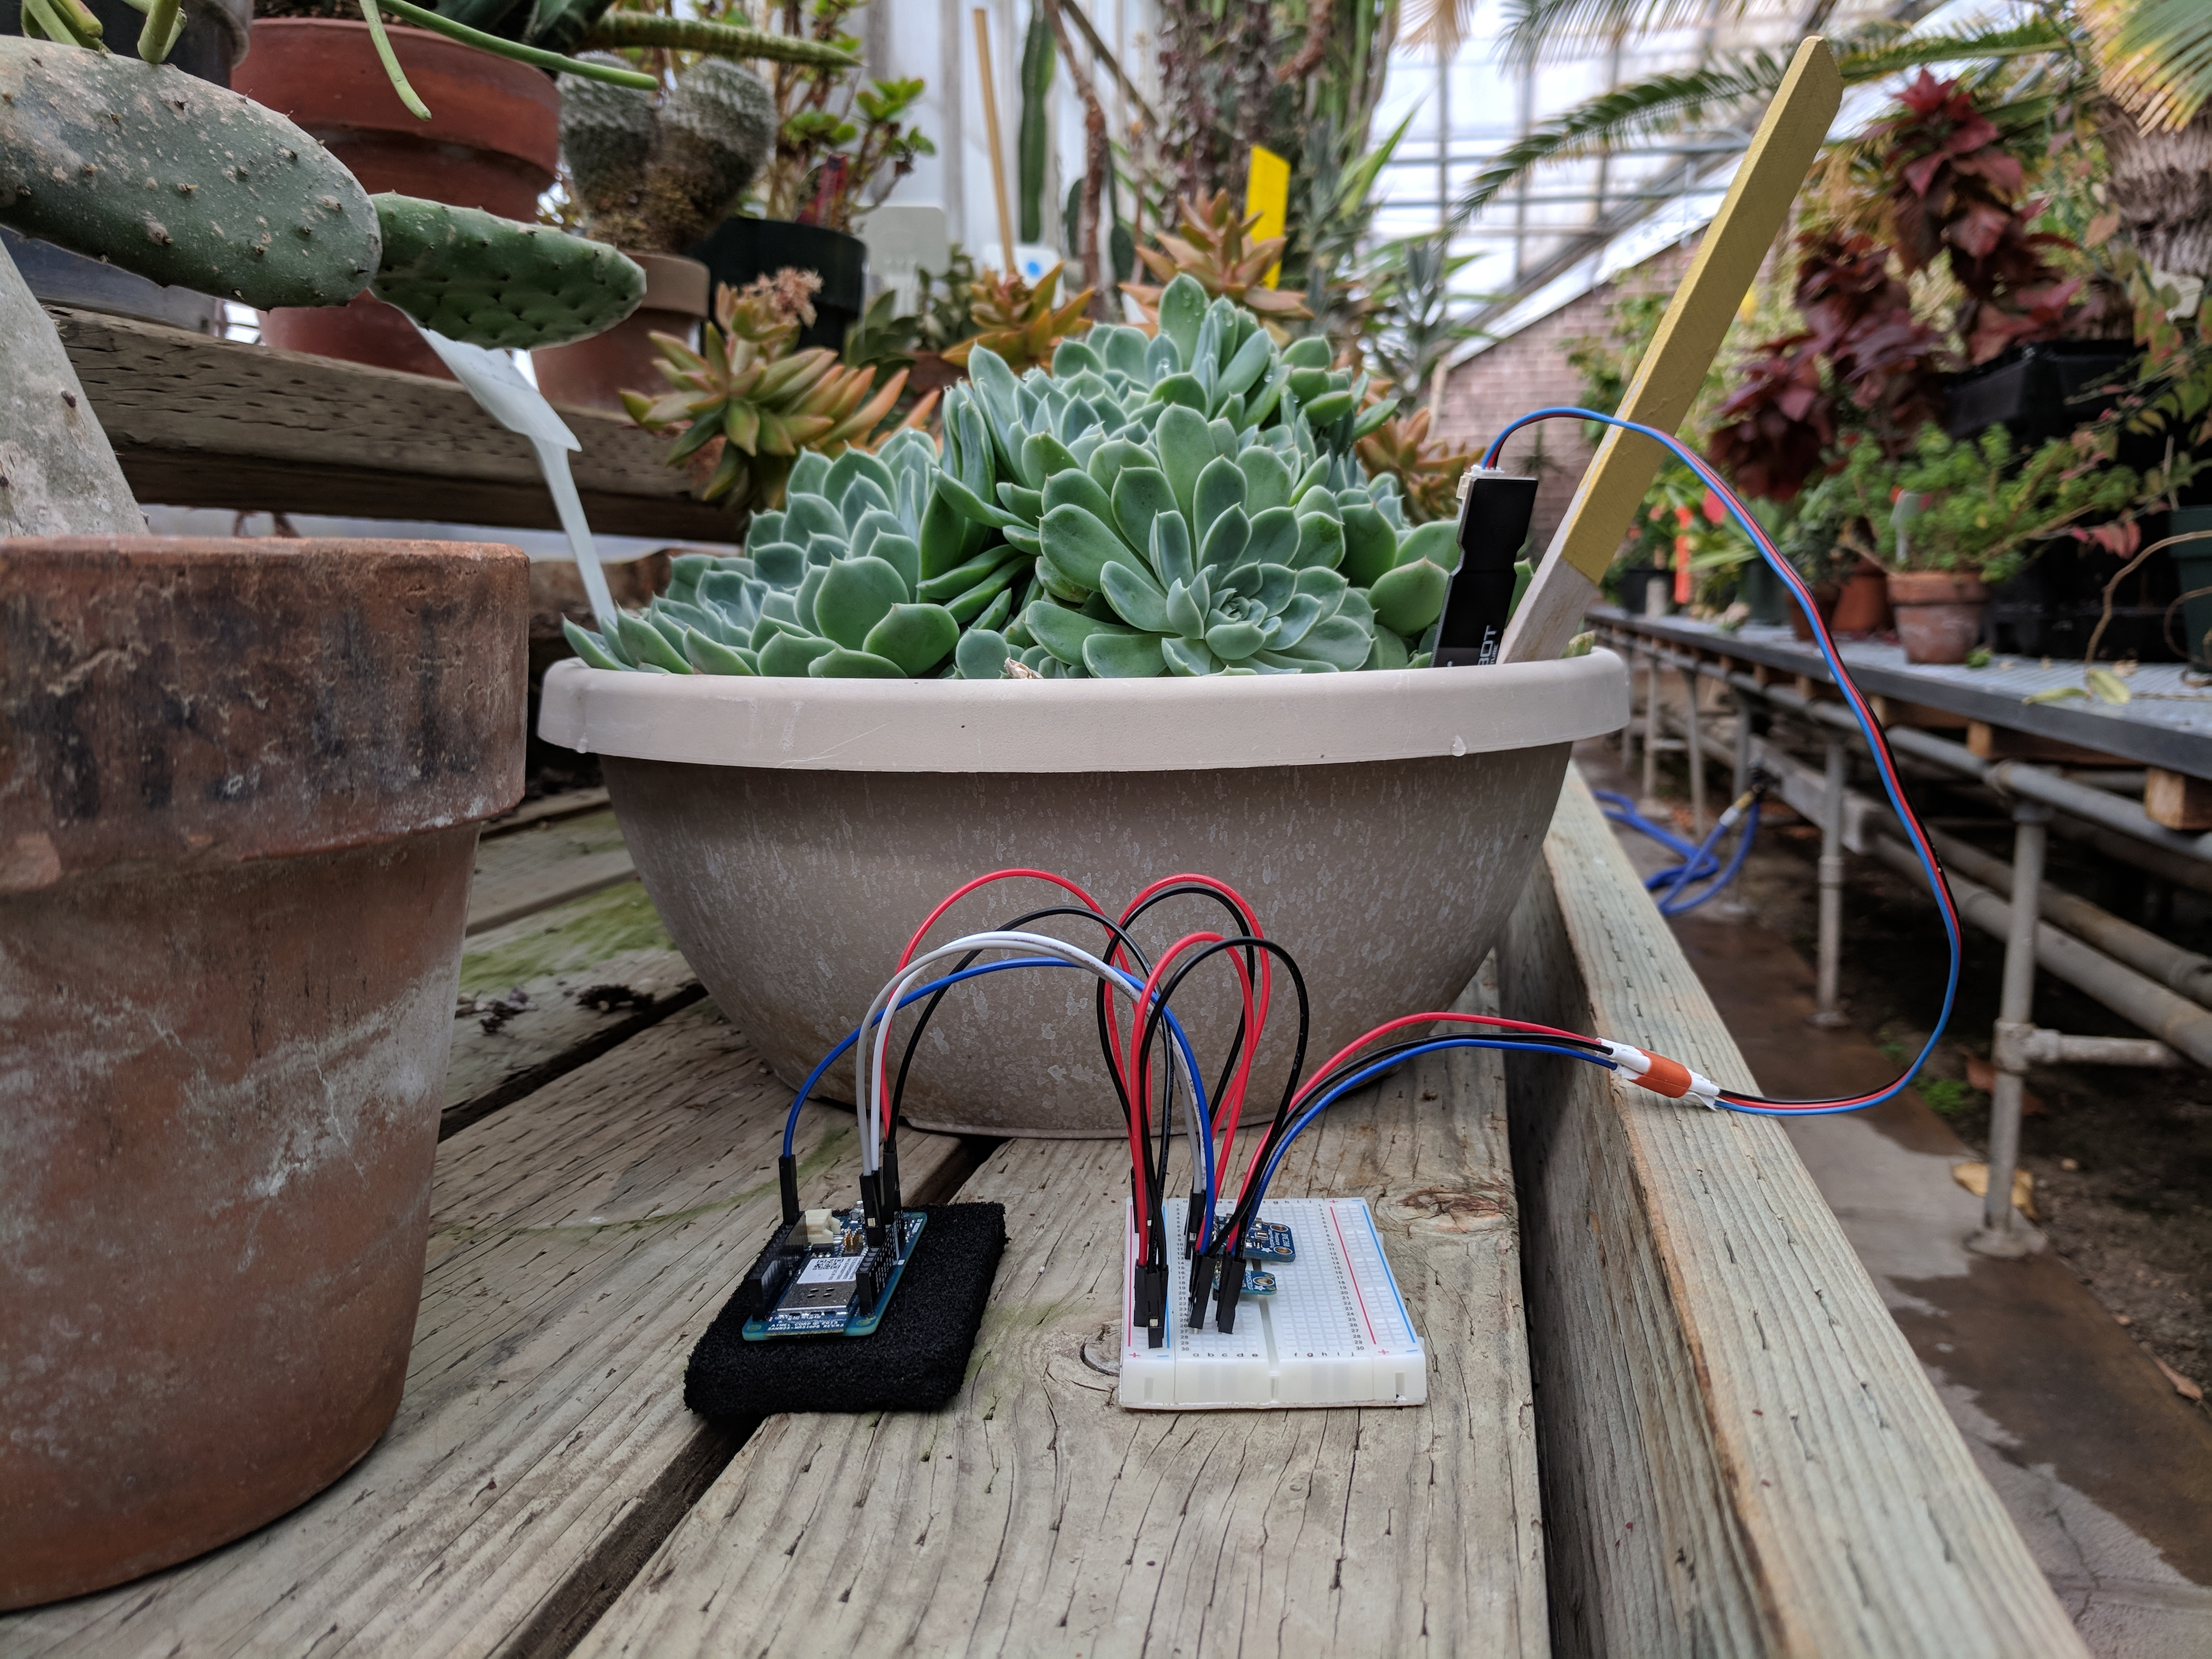
\includegraphics[width=0.5\textwidth]{green_house_testing}
\end{figure}

\begin{figure}[H]
  \caption{GS2: The MKR1000 board}
  \centering
  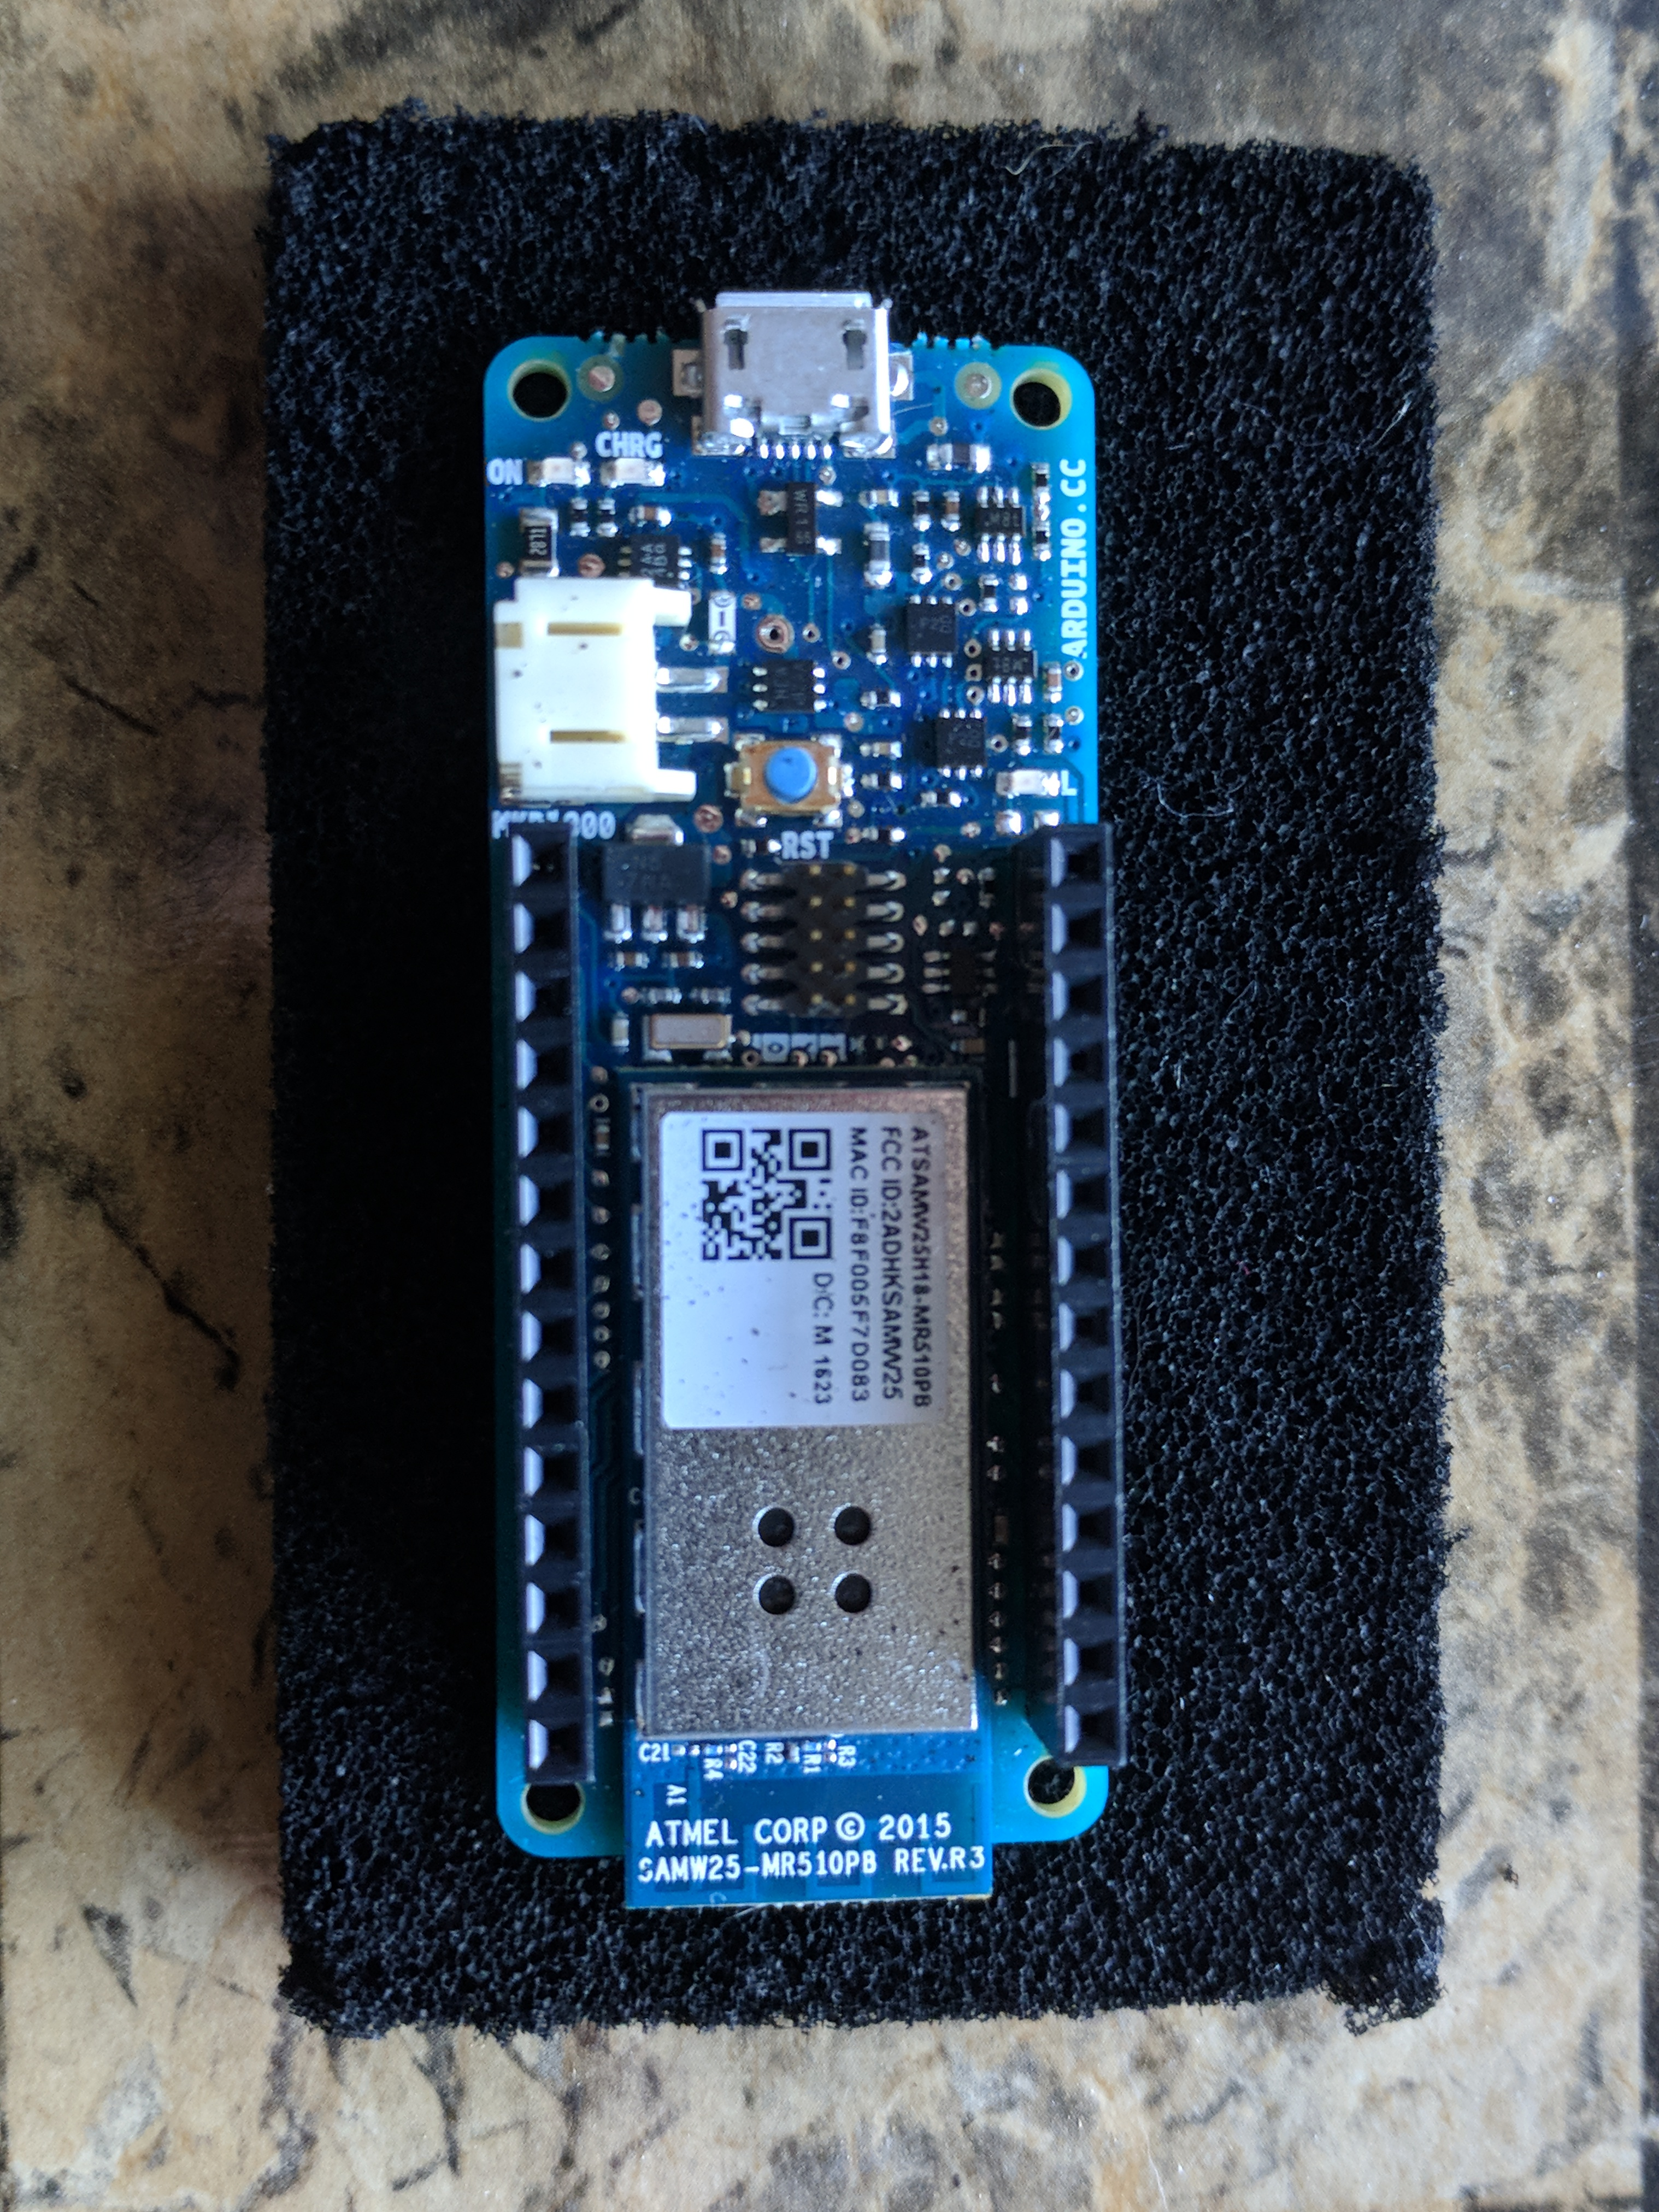
\includegraphics[width=0.5\textwidth]{MKR1000}
\end{figure}

\begin{figure}[H]
  \caption{GS2: Air and Light Sensors}
  \centering
  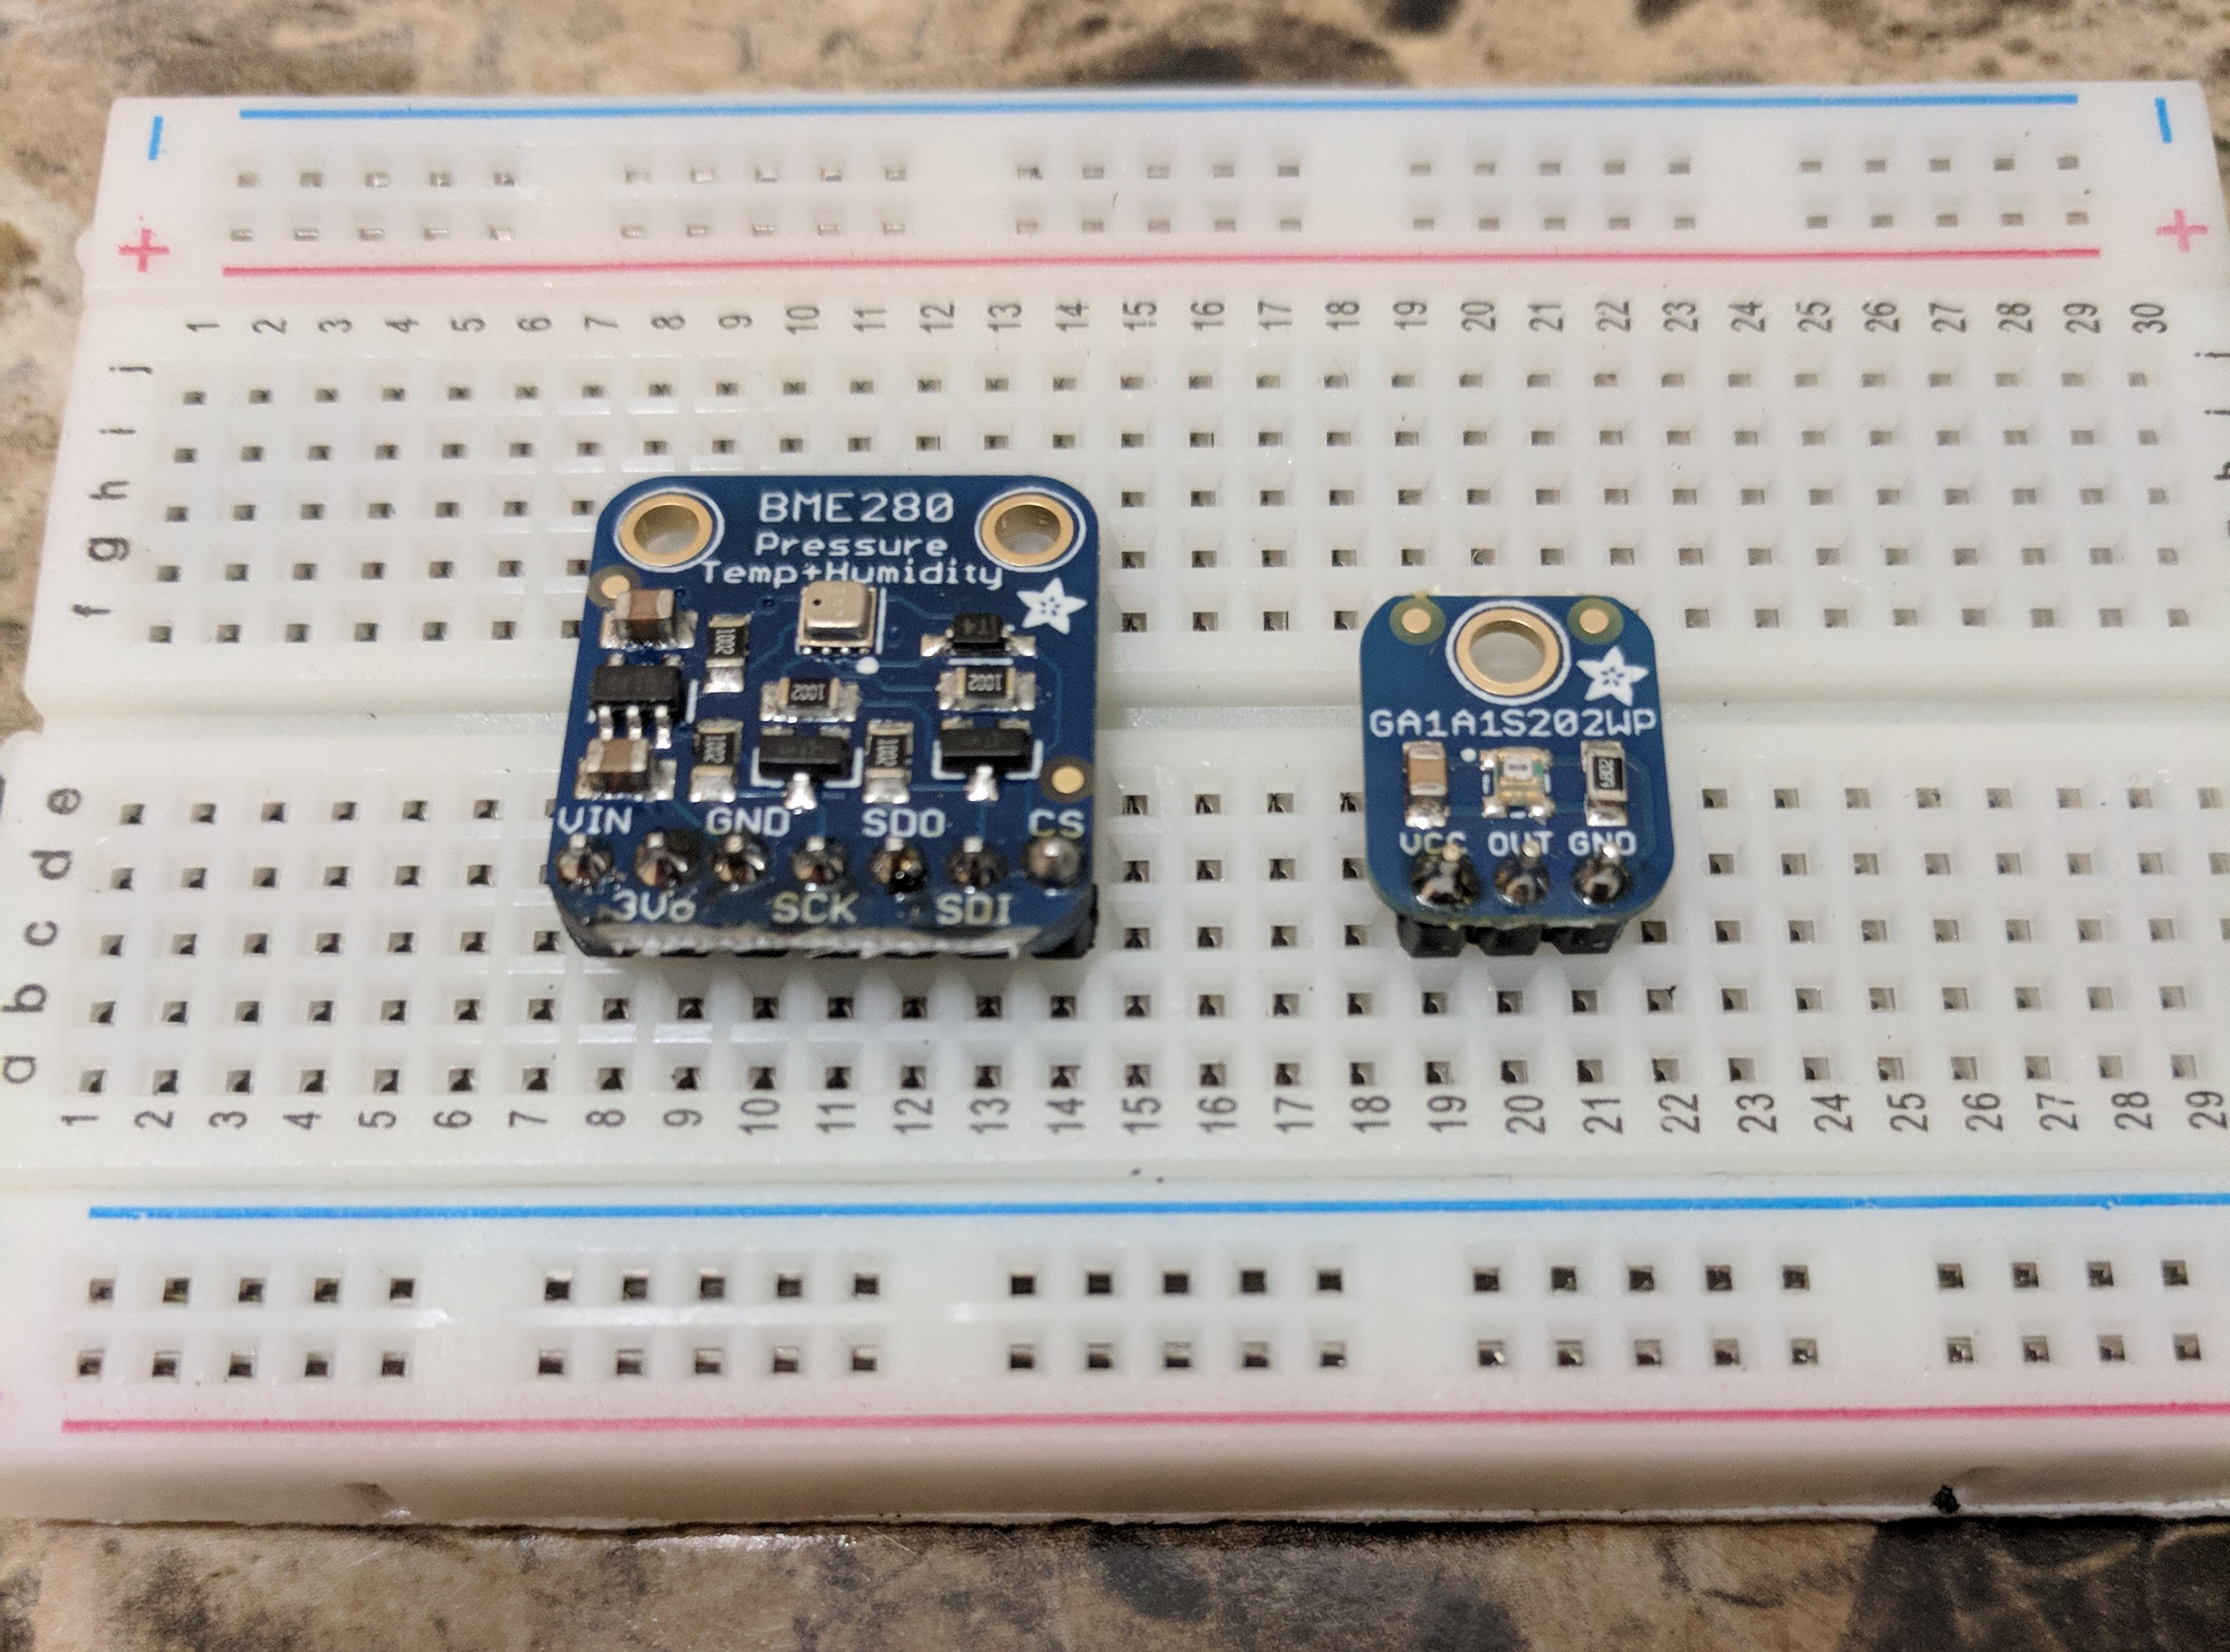
\includegraphics[width=0.5\textwidth]{air_light_sensors}
\end{figure}

\begin{figure}[H]
  \caption{GS2: Soil Moisture Sensor}
  \centering
  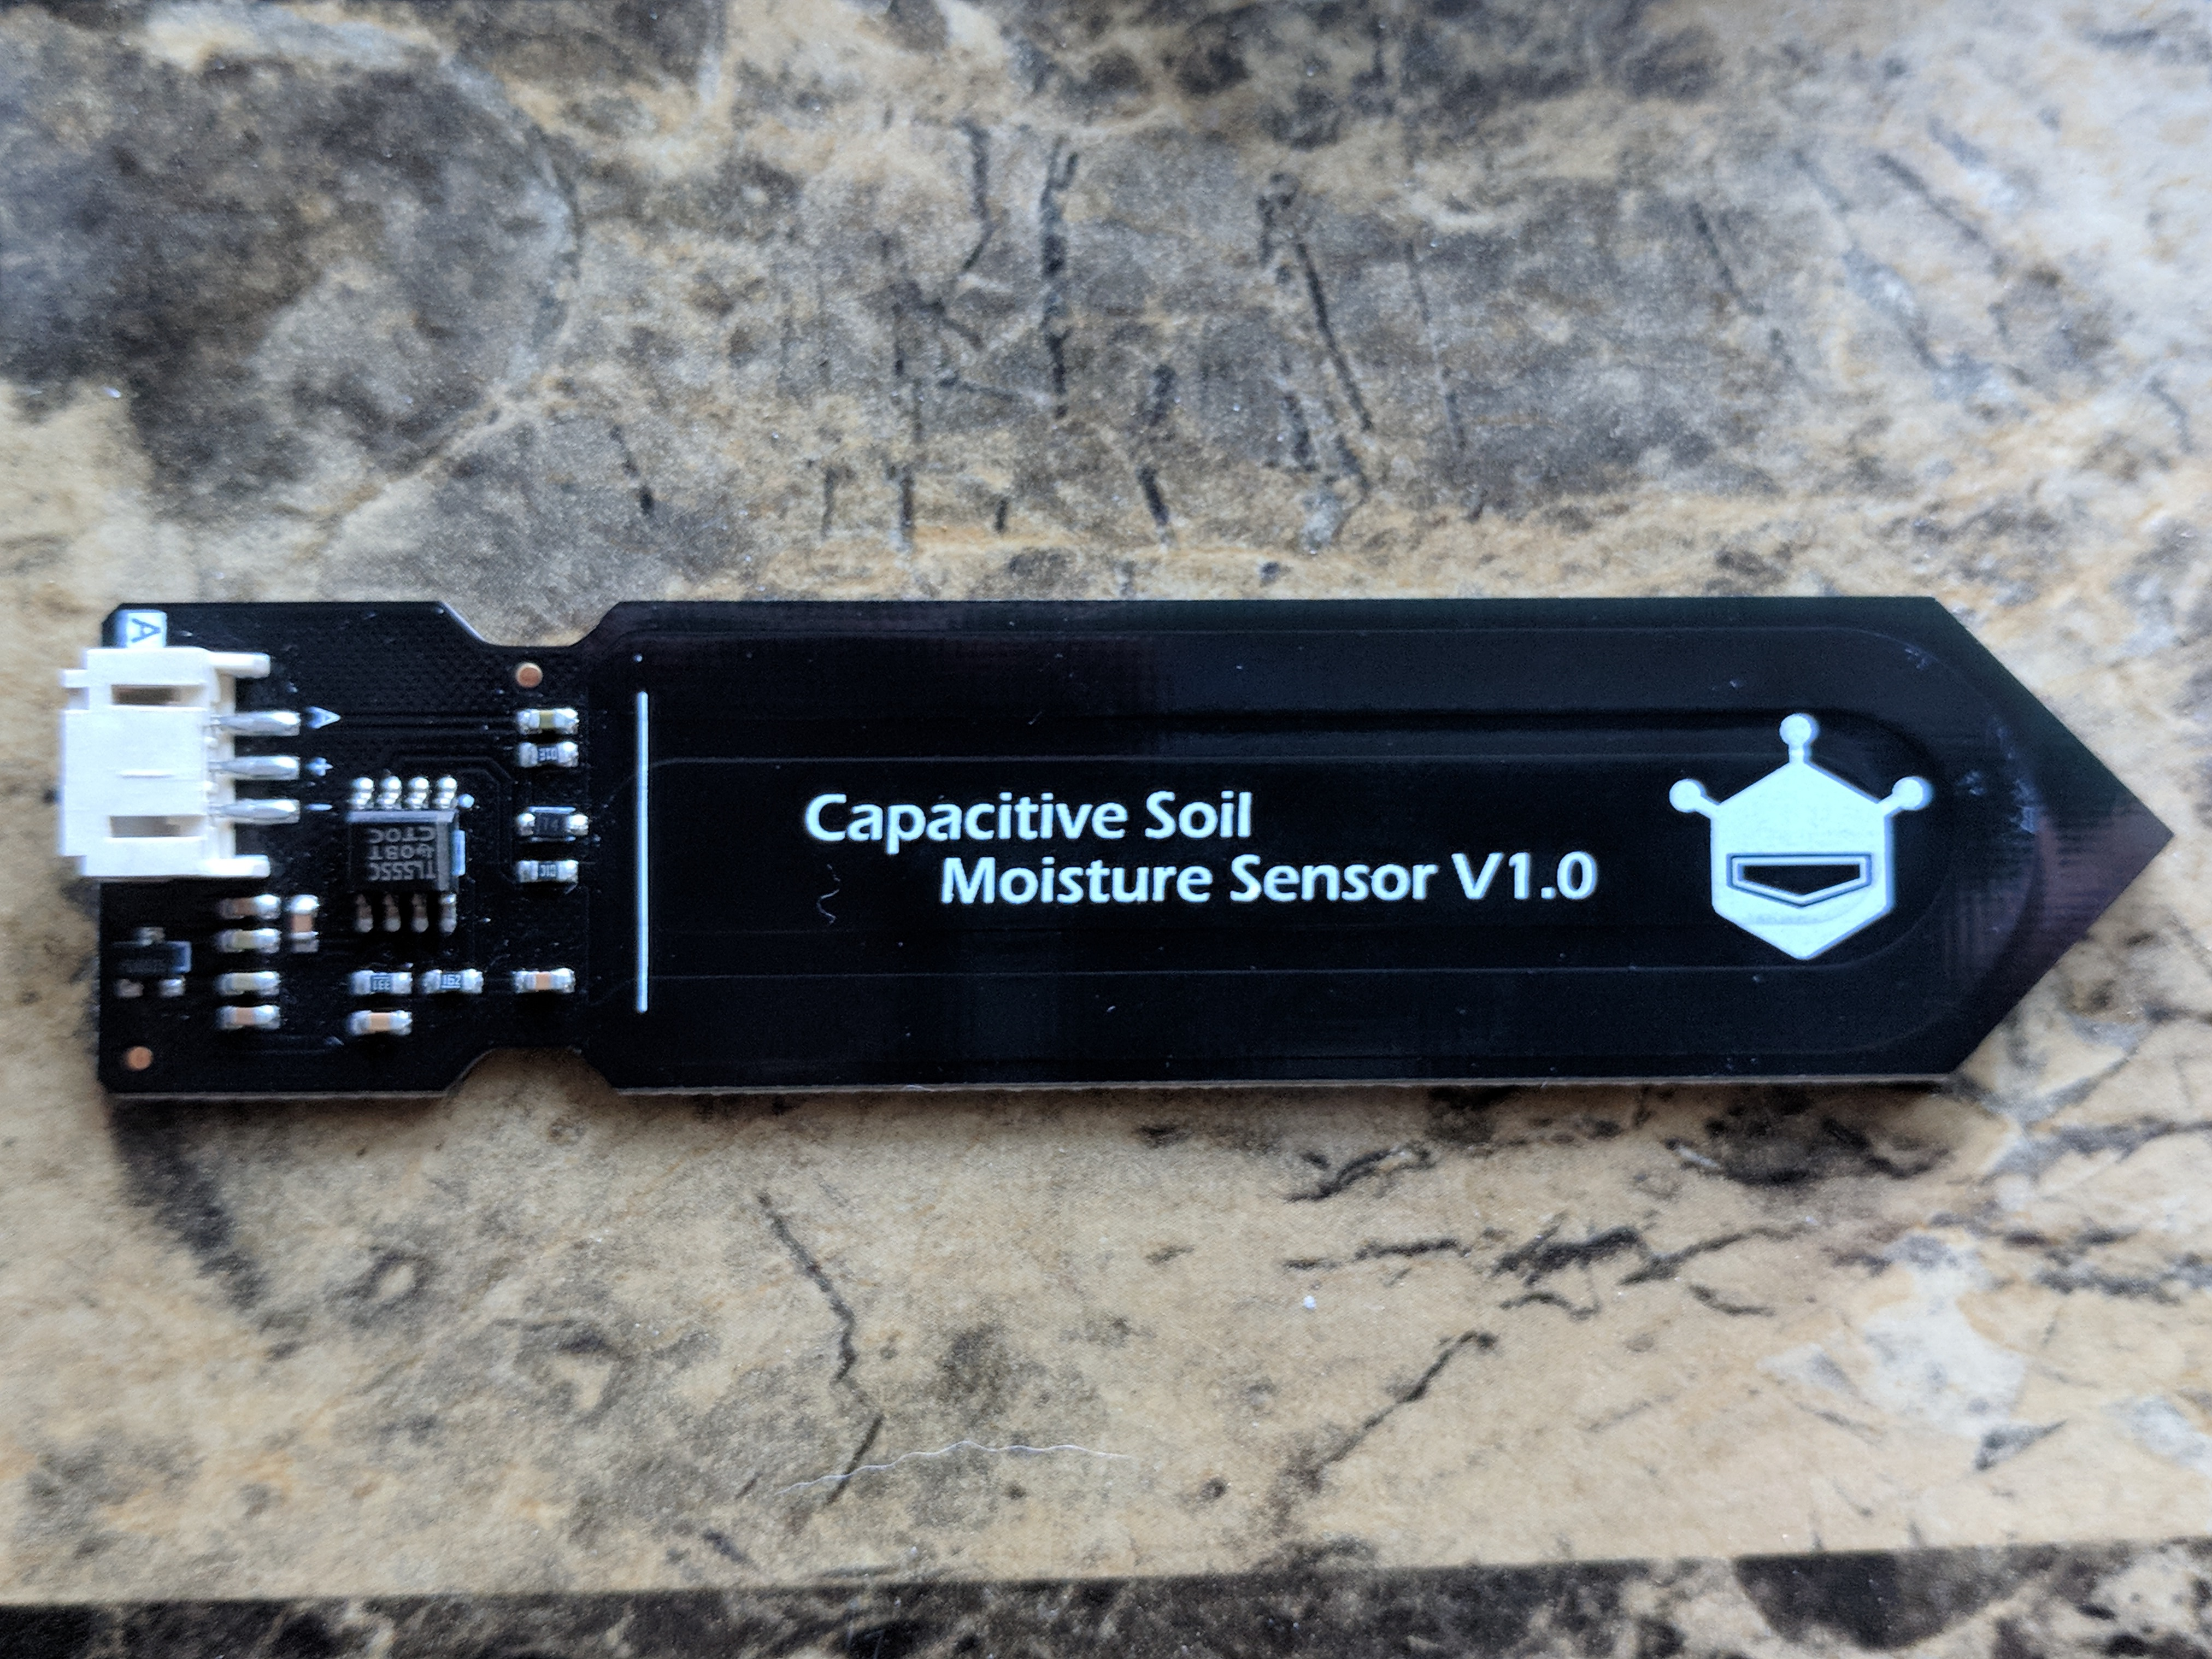
\includegraphics[width=0.5\textwidth]{soil_sensor}
\end{figure}

\section{Jack Neff}

\subsection{Purposes and Goals}

\subsubsection{Remote Access}
One of the main high-level purposes of the GS2 is to allow users to monitor conditions on their farm without having to go out and check the device itself. The goal here is achieved by hosting a web page and database on Google Cloud Platform that interfaces with the device, and displays/stores data that the device sends. An additional goal added later in development at the request of the clients was "two-way communication", in which the web site is capable of sending data in addition to receiving, allowing users to change the interval at which the device collects data from a page on the web site.

\subsubsection{Provide Information}

Chiefly, the GS2 is intended to keep the user updated about the conditions on their farm. If the user wants to look up the current conditions, that should be easy, as should looking up the conditions from a month ago. To achieve this purpose, the design goal has been to display all data simply and clearly on the homeage of the web site, and to implement a search functionality that searches the database for a specified time interval, then graphs it. On top of monitoring conditions in real time, the system uses a database to store up to years worth of collected data, the system will give users the capability of in-depth analysis into the correlation between weather conditions and crop quality, and allow them to hone their growing practices. 

\subsubsection{Cloud Platform}

The GS2 is intended to operate on a cloud server, so that it is easily portable and scalable for larger farms. From the beginning, my goal has been to host both the database and web site on the Google Cloud Platform (GCP), since it has those advantages, and provides a free trial. To accomplish this goal, I needed to rent some CPU time on a Google server and deploy a virtual machine, then install the appropriate software. 

\subsection{Where We Are At Now}

\subsubsection{Database}

The MySQL database is finalized and may not be updated for the duration of the project. It contains two tables, one for rows of data from the sensors, and one that holds information about the system such as the read time and parameter bounds. It is part of a LAMP (Linux, Apache, MySQL, Perl) installation on the GCP virtual machine, and contains two tables. One for them contains rows of sensor data, and one stores system parameters. 

\subsubsection{Web Site}

The web site is in the final stages of completion. So far, I have created a homepage with graphs of the last 12 data readings from the sensors, one graph per environmental parameter. These are easy to read and understand, and are accompanied by some stats such as maximum value, or average of a parameter over the last 12 readings. These readings change color to alert the user when above or below user-specified upper and lower bounds, which can be manually set from a linked web page.

\subsection{Left To Do}

\subsubsection{Web Site}There are a few more features I want to add to the web site before it is done. I am not yet done with the search feature that allows the user to graph a custom set of data, although I am extremely close. This would appear on the homepage to the right of the graphs. I also want to add a 24-hour forecast, with data recieved from Accuweather monitoring services, which will be displayed to the left of the graphs. This was not an initial requirement but it is not difficult to implement and will be very helpful. Finally I want to possibly reformat the graph section of the homepage, to only show one graph at a time, with buttons that will switch from one to the other. If I have time, I may implement a notification system that stores notifications about out-of-bounds environmental conditions and provides an alert on the homepage when notifications are unread. If I don't have time, highlighting of out-of-bounds data in red or blue text will suffice.  

\subsection{Problems}

\subsubsection{Displaying Data}

To graph the data, I used an API called Fusioncharts, which requires data be fed to its render function in a specific key-value pair format. Getting the data into this format was one of the initial hurdles to rendering a graph. This was accomplished by iteratively filling two arrays, and then using the array\_combine PHP function. Another problem that has not been solved as of yet is the planned implementation of a bootstrap carousel, which displays a stack of images one at a time and allows users to cycle through them. These carousels have a reputation of being difficult to program in any case, and in our case the graphs aren't traditional images, which makes things even more difficult. The current solution to the problem graph selection is to show them all stacked vertically, with icons that when clicked, automatically scroll the page down to the corresponding graph. 

\subsubsection{Environmental Bounds}

The whole year we had planned to program a system that would indicate if the environment is, for example, too cold outside for the type of grapes you are growing, or not humid enough. If an environmental parameter is measured to be outside the preferred bounds, the reading would change color to red or blue, indicating that something is wrong. At first I faced this like a research problem, wanting to study the preferred conditions of grapes and factor them into the site design.  After a lot of analysis, I came to the conclusion that it is best if the bounds for the environment were left up to the user, and they are allowed to set them at any time to any value. This solution addresses the problem in a more comprehensive way given that vintners and other farmers grow a wide variety of crops, with different environmental preferences. Allowing users to tailor these bounds to their specific crop, and giving users the chance to set and study these bounds by providing environmental reading history spanning years, seems to us to be the best way to implement these indications. 

\subsubsection{Forecast}

To improve user experience, I have included a 24-hour forecast with real time weather data provided by Accuweather. With Accuweather, you simply obtain an API key and append it to the Accweather URL and then get the contents of the file at that URL. Data is received as a string. From what I've gathered, I could use jQuery to parse this string easily and obtain the 24-hour forecast. Since I know PHP much better, I wrote a routine to manually parse this string using PHP.

\subsection{User Study}
I devised a user study and watched eight users navigate the web site as I asked them to perfrom basic functionalities. Of the eight users, five were men and three were women. The average age among them was 54. The oldest was 66 and the youngest was 40. 


\begin{table}[!htbp]
\centering

\label{User study participants}
\begin{tabular}{lllll}
Age & Sex & Job Title                                      & Browser & Internet Skill Level (Self rated, out of 10) \\
60  & M   & Lawyer, Haglund Kelly Law                      & IE      & 7                                            \\
59  & F   & Director of Public Relations, Waste Management & IE      & 7                                            \\
65  & M   & Regional Sales Director, Rubbermaid            & Chrome  & 8                                            \\
63  & F   & Stay-at-home Mother                            & Chrome  & 6                                            \\
47  & M   & Managing Director, ACM Wealth Managment        & Chrome  & 8                                            \\
42  & M   & Project Lead, Microsoft                        & Edge    & 9                                            \\
41  & F   & Sales Partner, Tableau                         & Safari  & 7                                            \\
63  & M   & Technical Fellow, Boeing                       & Chrome  & 9                                                   
\end{tabular}
\caption{Participants in user study}
\end{table}


\begin{figure}
  \caption{Homepage View as of 05-06-2018}
  \centering
    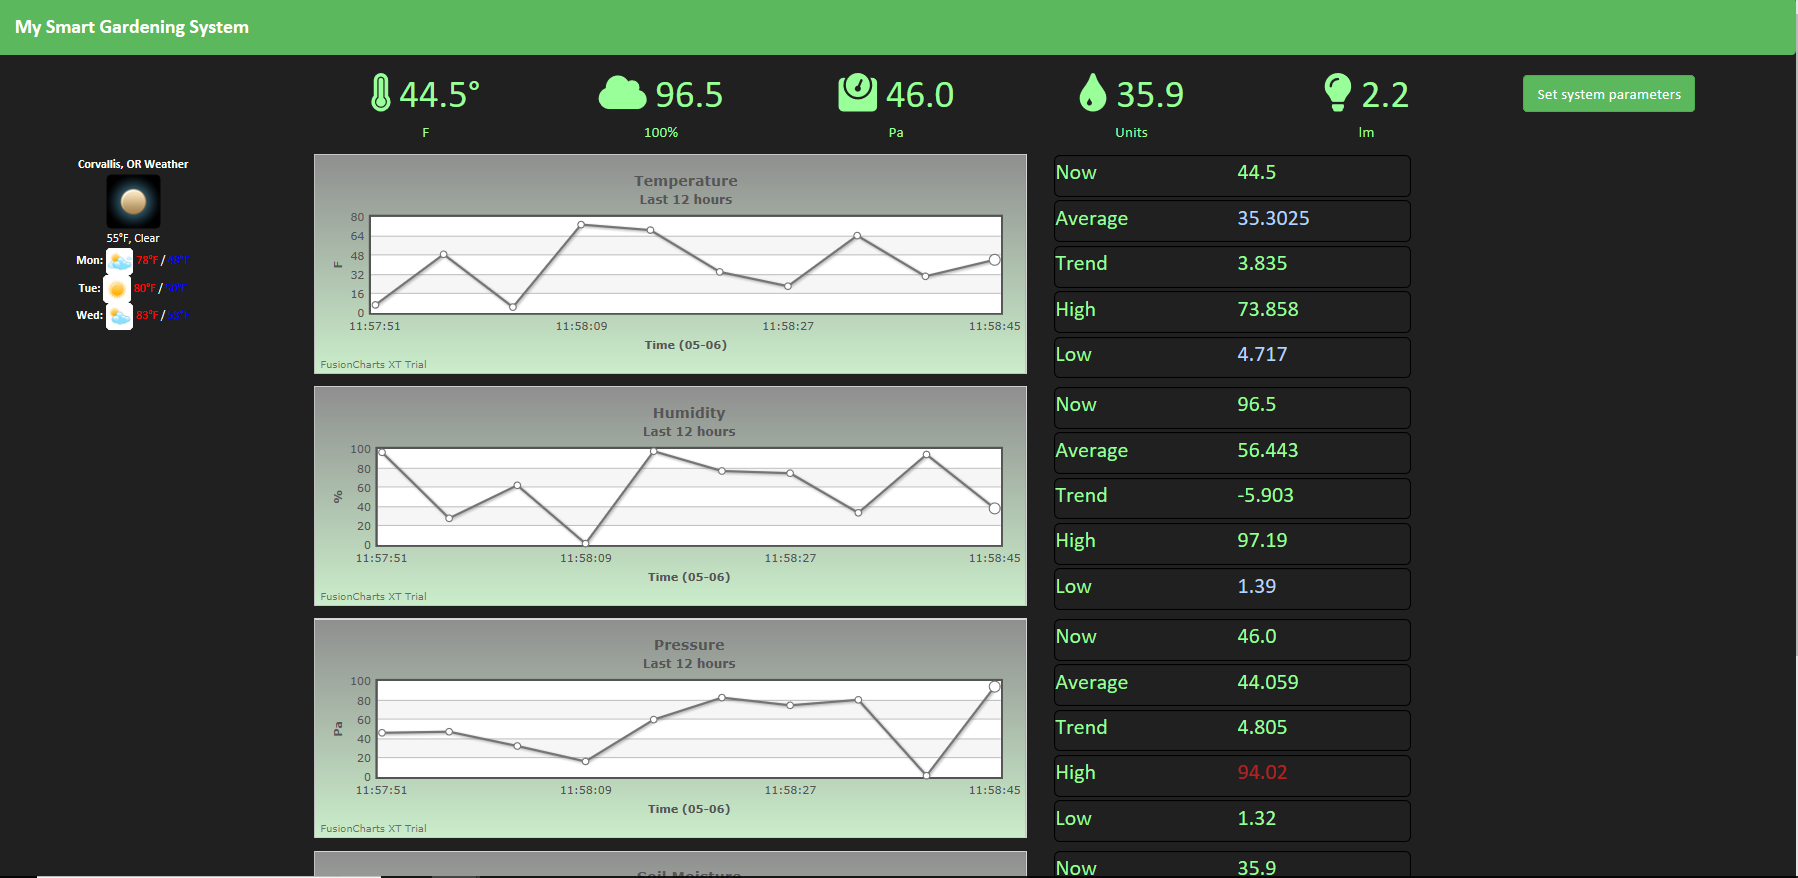
\includegraphics[width=0.7\textwidth]{homepage}
\end{figure}

\subsubsection{User Study Steps}

\paragraph{I want to find the graph of x}

Users were directed to the home page and asked to locate a random graph. Most found the correct graph within 10 seconds. Two users could not find the graph for over 20 seconds. Only one user used the linked icons at the top of the page to find the correct graph. 

This indicates that while in general any graph is still easy to locate, the current method of linked icons to facilitate this is not intuitive, and should be updated. A carousel for graphs is still an option, if it can be designed in bootstrap. If a carousel is not used, then a single-graph view will most likely be set up, with selector buttons to choose the graph to display. 

\paragraph{I want to find the most current reading of the x environmental condition}

Still on the home page, users were asked to locate a random current reading, such as the current humidity. Six of eight users were able to find the reading in under 10 seconds. Only one of eight took over 20 seconds. However, four users first answered with an incorrect reading, for some parameter other than the one that had been requested. This is likely because there are no text labels on the current readings, only icons, and users are unclear at first sight as to what those icons represent. The pressure icon, which is supposed to be a barometer, was referred to as a "clock" twice. On one users screen, data values were being incorrectly placed on the page due to a margin error. 

The take away here is that the current values, which are prominently displayed at the top of the page, need additional labeling, and the margins of the data values adjacent to the graphs need to be reformatted.

\paragraph{I want to update the x parameter for the system}

Now users were told to update a random parameter. The green "Set System Parameters" button on the right side of the home screen takes users to a linked page where parameters can be changed. However, very few users (only two of eight), were able to successfully navigate to the set parameters page and change a parameter within a full minute. Most users were confused because they did not see the linked button, or did not connect the label of the button to the idea of changing a parameter. Two users clicked on the numbers and labels displayed to the right adjacent to the graphs in an attempt to change the parameter. Three users actually clicked on the graph itself. If users could not navigate to the correct page in under a minute, they were assisted and able to navigate to the page.

Once on the set parameters page, many users were confused by the setup of the form. One remarked that "New and Current" did not make sense to them as labels, and suggested either "new and old" or "current" and "update." Two users noted that the phrase "Environment Parameters" made little sense to them, an d four noted confusion about the subtitle, which references the homepage. seven of eight users hit "enter" rather than the "Save changes" button to submit the form.

As a whole this was the most difficult task, and warrants the most edits. Clearly the link to the parameters page must be made both clearer as to it's significance, and larger so that it can be more easily seen. In addition, the graphs and their accompanying data were intuitive places for several users to look for the information they were seeking. If this pattern persists among other users, these assets could be linked to the parameters page as well as the aforementioned button. The parameters page's labels will need to be rewritten, probably from "current, new" to "old, new", given a new subtitle and possibly a new title. This challenge in particular points to a larger issue in the user interface that is it is quite technical. Steps will be taken to make it more user friendly before the May 11 deadline. Maybe most interestingly about this task was that all but one user hit enter, rather than clicking on the button. The javascript code covering the submission was only set to go off on a button click, and as a result did not execute. This will need to be fixed immediately. 

\paragraph{Additional thoughts/ideas}

Rating the site's appearance and ease of user on a scale of 1/10, the eight users who participated in the study gave a 7.9 rating for the appearance of the site, and a 5.7 un ease of use. Here are some additional suggestions and observations from users: 

\begin{itemize}  
\item The date under the graph should be changed from (05-04) to (May-04) or (05-04-2018).
\item A stronger indicator of success should be used to indicate a parameter change, like an alert box with "Success!!!" in it. 
\item The term "bound" is confusing should be changed to "range" wherever it is used.
\item The graph timeframes are labeled incorrectly. They read: "Last 12 hours", but the interval is not always an hour, it just shows 12 points (this is true and will be fixed shortly).
\item Margin of graph metadata needs to be fixed so that the value and label are on the same line.
\end{itemize}


\section{Jiayu Han}

\subsection{Recap}

Based on the vision from Intel, we plan to create a device based around the vineyard in Oregon that can simplify aspects of gardening and provide the users with more in-depth analysis of the vineyard. Our project, Green Smart Gardening System, is a solar energy powered Internet-of-Thing(IOT) device that monitors and analyses the environmental conditions, including temperature, air moisture, pressure, soil moisture and the light.

We design our project with 9 different requirements. The fields, which I selected at the beginning of this one-year project, are wireless connection, power system and packaging.

\subsection{Where I Am}

\subsubsection{Wireless Connectivity}

Wireless connection was one of the priority of our requirements for the project. The two unique features about our project are that our device is green energy powered and it is an IOT device. The most determining factor for us to pick Arduino MKR1000 micro-controller is that it has built-in Wi-Fi module. 

By the beginning of the last term, we already had the Wi-Fi code setup. There is already Wi-Fi101 library for MKR1000 to build the Wi-Fi connection. The only problem we had was that we were not able to connect to the internet which requires a web-page log-in system. However, that does not really affect the wireless connection since most consumer Wi-Fi do not require web-page to connect to. 

\subsubsection{Power System}

As we mentioned above, the green energy is one of our unique features about our project. We designed to plug both solar panel and battery into the MKR1000 to make our project become a solar energy powered device. Based on the Oregon weather, our power system design requires both solar panel and large capacity battery/battery bank to provide power even during the long rainy season in Oregon.

The power system was started right after the wireless connection. It was mainly research about the MKR1000, solar panel and the battery. After all the research, we were able to confirm that the MKR1000 was capable of using two different power source and has automatically switch. We started the testing with a 6V 6W solar panel and a standard 21000mAh battery bank, since there is mini-USB port provided on MKR1000. We did not find out later that the battery bank had a complicated problem which conflicted the way we want the device to run. At the beginning of this term, the problem was solved by switching to Li-ion batteries instead of battery bank with more testing. As for now, we have already finished demo for power system to show the MKR1000 built-in automatic switch process for the power system.

\subsubsection{Packaging}

Our plan for the device was originally pack everything into the same package with the solar panel on top of the package to gather the maximum illumination, and the soil moisture sensor would be partially out of the package to collect the data. In this case, we could keep our device to be compact and outdoor friendly. 

The package design process started by the middle of the 2018 Winter term. Our client, Intel, preferred 3D printing for the packaging which provides high modifiability. Since I have no experience in 3D model, I spent couple weeks to learn the 3D model tool, Google Sketchup. Based on the information we collected from the vineyard tour and the dimension limitation of the 3D printer, we adjusted the 3D model design from all-in-one to 3 separate packages. One is the main package for the MKR1000, breadboard and most sensors; one is specifically for the soil moisture sensor since it needs to be deep under the ground; the last one is for solar panel and battery because of the solar panel size. Later, I added the tolerance for the 3D model required by the client. As for now, we currently have the printed 3D packaging, though there are some minor adjustments need to be made. 

\subsection{What's Left}

At this stage, the requirements for the wireless connection, power system and the packaging are mostly finished. We already have the printed 3D model and the power system demo. There are only two more things to be done to perfect our project. Because of the limitation of 3D printer, the packaging had some minor errors. We are planning to improve the 3D model based on the current 3D print we have. The second thing will be testing the full device with a long run to examine any possible problems.

\subsection{Problems}

In the power system, we originally picked the battery bank as the energy storage, because of its modularity, high capacity and compatibility. However, we found out later that the battery banks we could find on the market were too “advanced”. Almost all of them have a built-in logic that they will shut down when the device connected is fully charged or not requiring power after a period and requires user to physically press the power button to turn the power bank on. It conflicts with our board logic which the device only collects data once a while and will be in sleep mode during that time. The device will also be using solar panel as the primary power source when there is enough illumination provided. We had some ideas with the battery bank, however, they were either too complicated or useless. We end up solve the problem by switch to rechargeable Li-ion batteries and changed the port for both solar panel and the battery.

\subsection{Images}

\begin{figure}[H]
  \caption{Power System Demo Setup}
  \centering
  \includegraphics[width=0.5\textwidth]{power_setup}
\end{figure}

\begin{figure}[H]
  \caption{3D model for the packaging and MKR1000 stand}
  \centering
  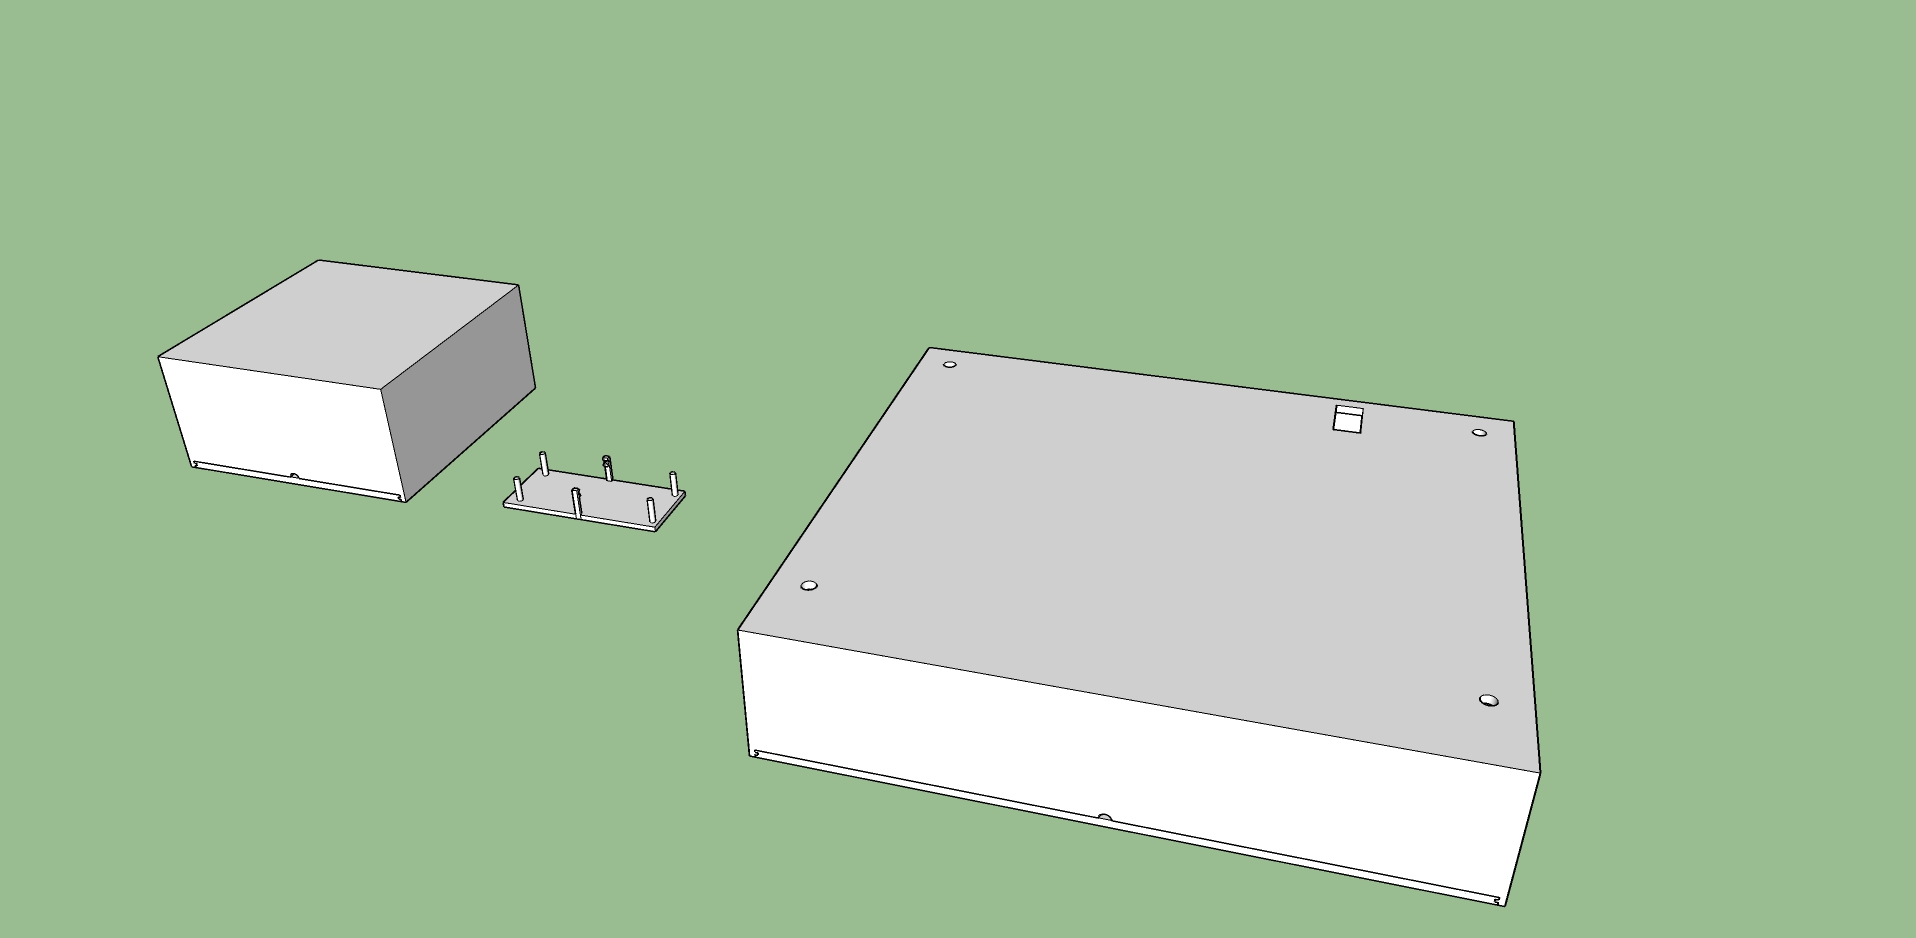
\includegraphics[width=0.5\textwidth]{packaging}
\end{figure}


\section{Conclusion}

This document covered many of the events that happened for the first portion of the term. We addressed the work that we are each responsible for in our project. From there we noted where we were on these tasks, and what we had left to do. Then, any problems that were dealt with over the duration of this term were acknowledged.

\end{document}